\section{Conclusions}
In this work, we demonstrate and quantitatively analyse one type of spurious responses existing in both linear and non-linear dynamic analysis of vibrating systems that stems from linear interpolation of input load. Within the scope of seismic engineering, typical values are chosen to illustrate the issue. It is worthing emphasising that the identified issue exists in all systems as long as linear interpolation is used, regardless of parameters (sampling frequency of input, material properties of system, natural frequency distribution, etc.).

\begin{figure}[htb!]
\centering\footnotesize
\tikzstyle{label}=[rectangle,rounded corners,minimum width=3cm,minimum height=1cm,text centered,draw=black,fill=gray!20]
\tikzstyle{exp}=[rectangle,rounded corners,minimum width=2cm,minimum height=1cm,text centered,draw=black,fill=gray!10]
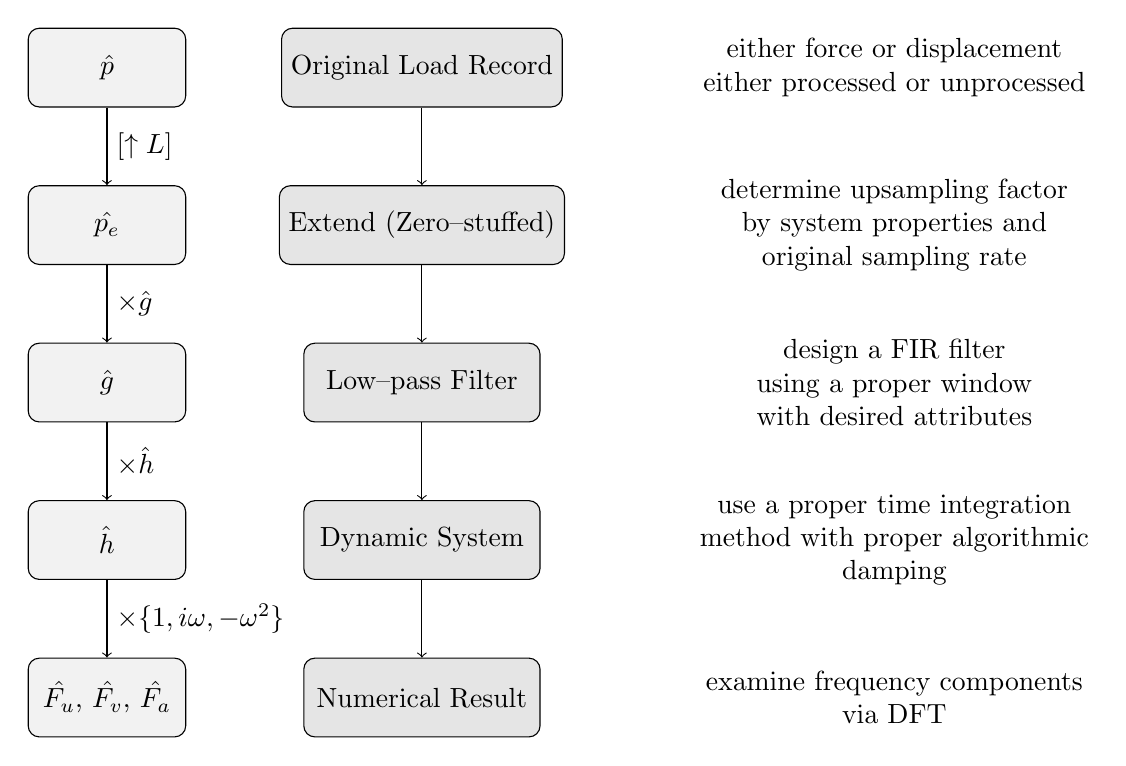
\begin{tikzpicture}
\node(original)[label]{Original Load Record};
\node(extended)[label,below of=original,yshift=-1cm]{Extend (Zero--stuffed)};
\node(filter)[label,below of=extended,yshift=-1cm]{Low--pass Filter};
\node(oscillator)[label,below of=filter,yshift=-1cm]{Dynamic System};
\node(system)[label,below of=oscillator,yshift=-1cm]{Numerical Result};
\draw[->](original)--(extended);
\draw[->](extended)--(filter);
\draw[->](filter)--(oscillator);
\draw[->](oscillator)--(system);
\node[xshift=5cm,right of=original,align=center]{either force or displacement\\either processed or unprocessed};
\node[xshift=5cm,right of=extended,align=center]{determine upsampling factor\\by system properties and\\original sampling rate};
\node[xshift=5cm,right of=filter,align=center]{design a FIR filter\\using a proper window\\with desired attributes};
\node[xshift=5cm,right of=oscillator,align=center]{use a proper time integration\\method with proper algorithmic\\damping};
\node[xshift=5cm,right of=system,align=center]{examine frequency components\\via DFT};
\node(p)[exp,xshift=-5cm,right of=original,align=center]{$\hat{p}$};
\node(pe)[exp,xshift=-5cm,right of=extended,align=center]{$\hat{p_e}$};
\node(g)[exp,xshift=-5cm,right of=filter,align=center]{$\hat{g}$};
\node(h)[exp,xshift=-5cm,right of=oscillator,align=center]{$\hat{h}$};
\node(f)[exp,xshift=-5cm,right of=system,align=center]{$\hat{F_u}$, $\hat{F_v}$, $\hat{F_a}$};
\draw[->](p)--(pe)node[midway,right]{$[\uparrow{}L]$};
\draw[->](pe)--(g)node[midway,right]{$\times\hat{g}$};
\draw[->](g)--(h)node[midway,right]{$\times\hat{h}$};
\draw[->](h)--(f)node[midway,right]{$\times\{1,i\omega,-\omega^2\}$};
\end{tikzpicture}
\caption{typical analysis flow with recommendations}
\end{figure}

It is evident that the linear interpolation is not ideal.
\begin{enumerate}
\item In order to avoid linear interpolation, it is better to have the identical time step size and sampling interval. To this end, one shall first choose a proper time step size that would be used in numerical analysis, typically it is smaller than sampling interval. Then, the seismogram shall be upsampled.
\item The low--pass filter shall possess sufficiently small side lobe level.
\item The high frequency noise exists intrinsically and is spotted analytically. Algorithmic damping can alleviate the issue but only to a limited degree.
\end{enumerate}

\begin{enumerate}
\item Determine whether the seismograph, in the form of either displacement or acceleration, is properly processed. Typical seismographs are preprocessed by applying a band--pass filter with bounds at around \SI{0.05}{\hertz} and \SIrange{25}{50}{\hertz} for structural analysis.
\item Determine a proper time step size and the corresponding upsampling ratio.
\item Design a proper upsampling filter so that time step size matches upsampling interval.
\item Avoid high frequency modes in the target structure. For example, use a properly integrated consistent mass matrix or full ranked diagonal mass matrix, limit the penalty factor within a reasonable range when it comes to model, for example, axial inextensibility. Constraints are better implemented via the Lagrange multiplier method.
\end{enumerate}

The numerical examples are carried out using \texttt{suanPan} \citep{Chang2022}. Scripts to generate figures and models can be found online.\footnote{\url{https://github.com/TLCFEM/dsp-dynamics}}